% Options for packages loaded elsewhere
\PassOptionsToPackage{unicode}{hyperref}
\PassOptionsToPackage{hyphens}{url}
\PassOptionsToPackage{dvipsnames,svgnames,x11names}{xcolor}
%
\documentclass[
  10pt,
]{article}
\usepackage{amsmath,amssymb}
\usepackage{iftex}
\ifPDFTeX
  \usepackage[T1]{fontenc}
  \usepackage[utf8]{inputenc}
  \usepackage{textcomp} % provide euro and other symbols
\else % if luatex or xetex
  \usepackage{unicode-math} % this also loads fontspec
  \defaultfontfeatures{Scale=MatchLowercase}
  \defaultfontfeatures[\rmfamily]{Ligatures=TeX,Scale=1}
\fi
\usepackage{lmodern}
\ifPDFTeX\else
  % xetex/luatex font selection
\fi
% Use upquote if available, for straight quotes in verbatim environments
\IfFileExists{upquote.sty}{\usepackage{upquote}}{}
\IfFileExists{microtype.sty}{% use microtype if available
  \usepackage[]{microtype}
  \UseMicrotypeSet[protrusion]{basicmath} % disable protrusion for tt fonts
}{}
\makeatletter
\@ifundefined{KOMAClassName}{% if non-KOMA class
  \IfFileExists{parskip.sty}{%
    \usepackage{parskip}
  }{% else
    \setlength{\parindent}{0pt}
    \setlength{\parskip}{6pt plus 2pt minus 1pt}}
}{% if KOMA class
  \KOMAoptions{parskip=half}}
\makeatother
\usepackage{xcolor}
\usepackage[margin=0.76in]{geometry}
\usepackage{longtable,booktabs,array}
\usepackage{calc} % for calculating minipage widths
% Correct order of tables after \paragraph or \subparagraph
\usepackage{etoolbox}
\makeatletter
\patchcmd\longtable{\par}{\if@noskipsec\mbox{}\fi\par}{}{}
\makeatother
% Allow footnotes in longtable head/foot
\IfFileExists{footnotehyper.sty}{\usepackage{footnotehyper}}{\usepackage{footnote}}
\makesavenoteenv{longtable}
\usepackage{graphicx}
\makeatletter
\def\maxwidth{\ifdim\Gin@nat@width>\linewidth\linewidth\else\Gin@nat@width\fi}
\def\maxheight{\ifdim\Gin@nat@height>\textheight\textheight\else\Gin@nat@height\fi}
\makeatother
% Scale images if necessary, so that they will not overflow the page
% margins by default, and it is still possible to overwrite the defaults
% using explicit options in \includegraphics[width, height, ...]{}
\setkeys{Gin}{width=\maxwidth,height=\maxheight,keepaspectratio}
% Set default figure placement to htbp
\makeatletter
\def\fps@figure{htbp}
\makeatother
\setlength{\emergencystretch}{3em} % prevent overfull lines
\providecommand{\tightlist}{%
  \setlength{\itemsep}{0pt}\setlength{\parskip}{0pt}}
\setcounter{secnumdepth}{-\maxdimen} % remove section numbering
\usepackage{amsmath,amssymb,mathtools}
\usepackage{booktabs,longtable,array}
\usepackage{graphicx,float}
\graphicspath{{/mnt/data/}}
\usepackage{xcolor}
\usepackage{hyperref}
\usepackage{microtype}
\definecolor{deepblue}{HTML}{1F4E79}
\hypersetup{colorlinks=true,linkcolor=deepblue,urlcolor=deepblue,citecolor=deepblue}
\setlength{\parindent}{0pt}
\setlength{\parskip}{5pt plus 1pt minus 1pt}
\renewcommand{\arraystretch}{1.15}
\ifLuaTeX
  \usepackage{selnolig}  % disable illegal ligatures
\fi
\usepackage{bookmark}
\IfFileExists{xurl.sty}{\usepackage{xurl}}{} % add URL line breaks if available
\urlstyle{same}
\hypersetup{
  pdftitle={RG-Improved Transient Matching and Explicit Thermal Collision Dynamics},
  pdfauthor={Technical Research Note v1.3},
  colorlinks=true,
  linkcolor={blue},
  filecolor={Maroon},
  citecolor={Blue},
  urlcolor={blue},
  pdfcreator={LaTeX via pandoc}}

\title{RG-Improved Transient Matching and Explicit Thermal Collision
Dynamics}
\usepackage{etoolbox}
\makeatletter
\providecommand{\subtitle}[1]{% add subtitle to \maketitle
  \apptocmd{\@title}{\par {\large #1 \par}}{}{}
}
\makeatother
\subtitle{Full Higgs-doublet multiplicities, log-resummed
selector-threshold matching, and an AMY-motivated quantum kinetic
replacement for BGK}
\author{Technical Research Note v1.3}
\date{18 August 2026}

\begin{document}
\maketitle

{
\hypersetup{linkcolor=}
\setcounter{tocdepth}{3}
\tableofcontents
}
\section{Executive verdict}\label{executive-verdict}

The v1.3 calculation produces a \textbf{pass for the resolved
RG-improved matching problem}, a \textbf{pass for the full Standard
Model colour and Higgs-doublet multiplicities at that loop order}, and a
\textbf{pass for replacing the BGK ansatz by an explicit
energy-conserving quantum collision kernel}. It remains a
\textbf{partial result for the exact LPM problem} and an \textbf{open
result for a non-Abelian two-time 2PI/Kadanoff-Baym evolution}.

The main matching result is that the enormous scale excursion found in
v1.2,

\[
\mathcal I_3(M/2)=102.407,
\qquad
\mathcal I_3(M)=6.57974,
\qquad
\mathcal I_3(2M)=-96.9351,
\]

is not a physical uncertainty. It is the explicit logarithm of a
fixed-order hard function before operator running and counterterms are
combined with it. At the resolved order,

\[
\boxed{
D_{FFS}^{\rm hard}
=
D_{FFS}^{\rm fixed}(\bar\mu)
+
\Delta_{\rm RG}(\bar\mu)
}
\]

is exactly independent of \(\bar\mu\) and gives

\[
\boxed{
\mathcal I_3^{\rm hard}=6.57973508149.
}
\]

Restoring the complete unbroken Higgs doublet gives two Yukawa channels
rather than the single-real-scalar proxy channel. Including that factor,
the relativistic vectorlike-colour contribution to \(g_*\), and one-loop
running from \(m_R\) to \(M\) gives

\[
\boxed{
C_3^{\rm full}=1.58896\times10^{-4}\ {\rm GeV}^2,
}
\]

and

\[
\boxed{
|\Delta V_{Qa}^{(3)}|
=4.2902\times10^3\ {\rm GeV}^4.
}
\]

This is still only

\[
\boxed{
3.053\times10^{-12}
}
\]

of the intended reheating-era finite-density focusing potential. The
multiplicity correction almost doubles the v1.2 proxy answer, but does
not threaten the mechanism.

After the explicit logarithm is removed, varying the lower matching
scale from \(M/2\) to \(2M\) changes the result only through ordinary
coupling and portal running:

\[
\boxed{
0.96469
<
\frac{C_3(\mu_D)}{C_3(M)}
<
1.03745.
}
\]

The kinetic calculation replaces the BGK relaxation ansatz by a discrete
gain/loss operator containing:

\begin{itemize}
\tightlist
\item
  six explicit \(1\leftrightarrow2\) channel families;
\item
  eight explicit \(2\leftrightarrow2\) channel families;
\item
  Bose enhancement and Pauli blocking;
\item
  Debye screening;
\item
  asymptotic thermal masses for \(H,D,q,g\);
\item
  an LPM formation-time kernel for collinear processes;
\item
  exact discrete energy conservation.
\end{itemize}

The implemented lattice contains \(514\) \(1\leftrightarrow2\)
transitions and \(14{,}289\) \(2\leftrightarrow2\) transitions. Starting
from an intentionally severe nonthermal Higgs pulse, it reaches \(99\%\)
of the equilibrium entropy gain by

\[
\boxed{
\tau_{99}\equiv Tt=3920.
}
\]

At the reheating temperature \(T=1.002\times10^8\,\mathrm{GeV}\), this
corresponds to

\[
\boxed{
\Gamma_{\rm kin}^{(99)}
=2.556\times10^4\,\mathrm{GeV}.
}
\]

Therefore,

\[
\boxed{
\frac{\Gamma_{\rm kin}^{(99)}}{\Gamma_R}
=1.729\times10^6.
}
\]

The tracked plasma is consequently an extremely fast subsystem relative
to reheaton and parent decays. For the homogeneous cosmological cascade,
replacing BGK by the explicit kernel is equivalent, to excellent
accuracy, to \textbf{adiabatically eliminating the kinetic distributions
after every energy injection}. The collision physics changes spectra and
microscopic entropy production, but not the sector total-energy
bookkeeping that fixes \(T_5/T_0\).

Full multiplicity also corrects the relativistic degrees of freedom:

\[
\boxed{
g_*=106.75+10.5=117.25.
}
\]

For fixed \(T_0=1.002\times10^8\,\mathrm{GeV}\) this changes

\[
\Gamma_R=1.47850\times10^{-2}\,\mathrm{GeV},
\qquad
\mu_H=1.92766\times10^4\,\mathrm{GeV}.
\]

Re-running the momentum cascade with this decay width gives

\[
\boxed{
B_5=0.00529888708,
\qquad
\tan\theta=0.0729871,
}
\]

for \(T_5/T_0=1/4\).

The strongest defensible conclusion is:

\[
\boxed{
\begin{gathered}
\text{the large matching-scale instability is removed by consistent RG completion,}\\
\text{the full doublet and colour multiplicities leave the transient correction tiny,}\\
\text{and explicit weak-coupling collision dynamics validates instantaneous plasma equilibration.}
\end{gathered}
}
\]

The next frontier is no longer BGK. It is the \textbf{numerical solution
of the full AMY transverse LPM integral equation and full-angle
\(2\leftrightarrow2\) phase-space integral}, followed by a
gauge-covariant non-Abelian two-time calculation.

\section{1. Model and full Standard Model
multiplicity}\label{model-and-full-standard-model-multiplicity}

\subsection{1.1 Resolved interaction
chain}\label{resolved-interaction-chain}

The relevant interactions are written schematically as

\[
\begin{aligned}
\mathcal L\supset{}&
-\frac12\left(m_R^2+\lambda_{QR}\mathcal Q\right)R^2
-\mu_H R H^\dagger H
\\
&-
\left[y_D\overline Q_L H D_R+\mathrm{h.c.}\right]
-M(a)\overline DD,
\end{aligned}
\]

where

\[
M(a)=M\left[1-\epsilon\cos\left(\frac a{f_a}\right)\right].
\]

The fields carry

\[
Q_L\sim(\mathbf3,\mathbf2,1/6),
\qquad
D_{L,R}\sim(\mathbf3,\mathbf1,-1/3),
\qquad
H\sim(\mathbf1,\mathbf2,1/2).
\]

At zero external momentum the three-loop 1PI but 2PR graph factorises
into:

\begin{enumerate}
\def\labelenumi{\arabic{enumi}.}
\tightlist
\item
  a one-loop selector-reheaton-Higgs kernel;
\item
  a two-loop fermion-fermion-scalar threshold kernel.
\end{enumerate}

The colour trace gives

\[
N_c=3.
\]

In the unbroken phase,

\[
y_D\overline Q_L H D_R
=
y_D\left(\overline u_LH^++\overline d_LH^0\right)D_R.
\]

There are therefore two complex Higgs/left-fermion channels.
Equivalently, decomposing the doublet into four real components gives
four vertices of strength \(y_D/\sqrt2\), and

\[
4\left(\frac{y_D^2}{2}\right)=2y_D^2.
\]

Relative to the one-real-scalar proxy,

\[
\boxed{n_w=2.}
\]

No additional electroweak gauge multiplicity enters this specific
resolved graph. Electroweak gauge corrections first enter through
running or through higher-loop matching graphs.

\subsection{1.2 Relativistic degrees of
freedom}\label{relativistic-degrees-of-freedom}

The vectorlike Dirac colour triplet contributes

\[
\Delta g_*
=\frac78(2_{\rm spin})(2_{D+\bar D})(3_{\rm colour})
=10.5.
\]

At \(T_R\gg M\),

\[
\boxed{g_*^{\rm full}=117.25.}
\]

This correction was absent from the earlier reheating benchmark.

\section{2. RG completion of the hard
function}\label{rg-completion-of-the-hard-function}

\subsection{2.1 Fixed-order expression}\label{fixed-order-expression}

Define

\[
x=M^2,
\qquad
z=m_h^2,
\qquad
r=\frac zx,
\qquad
\ell=\ln\frac{x}{\bar\mu^2}.
\]

The fixed-order mixed derivative is

\[
\begin{aligned}
D_{FFS}^{\rm fixed}(x,z;\bar\mu)
={}&
2\ln\frac{x}{z}
\ln\frac{x-z}{\bar\mu^2}
-
\ln^2\frac{x}{\bar\mu^2}
\\
&-
2\operatorname{Li}_2\left(\frac zx\right)
+
\frac{\pi^2}{3}.
\end{aligned}
\]

Its scale dependence is large because

\[
\ln\frac{M^2}{m_h^2}\simeq17.97.
\]

\subsection{2.2 Running contribution}\label{running-contribution}

The local operator evolution and counterterm matching supply

\[
\boxed{
\Delta_{\rm RG}
=
-2\ln\frac{x}{z}\,\ell
+
\ell^2.
}
\]

Adding the two gives

\[
\begin{aligned}
D_{FFS}^{\rm hard}(x,z)
={}&
2\ln\frac{x}{z}\ln(1-r)
-2\operatorname{Li}_2(r)
+
\frac{\pi^2}{3}.
\end{aligned}
\]

The verification suite proves symbolically that

\[
D_{FFS}^{\rm fixed}
+
\Delta_{\rm RG}
-
D_{FFS}^{\rm hard}=0
\]

and

\[
\bar\mu\frac{d}{d\bar\mu}
\left(
D_{FFS}^{\rm fixed}
+
\Delta_{\rm RG}
\right)=0.
\]

In the hierarchical limit,

\[
D_{FFS}^{\rm hard}\longrightarrow\frac{\pi^2}{3}.
\]

\begin{figure}
\centering
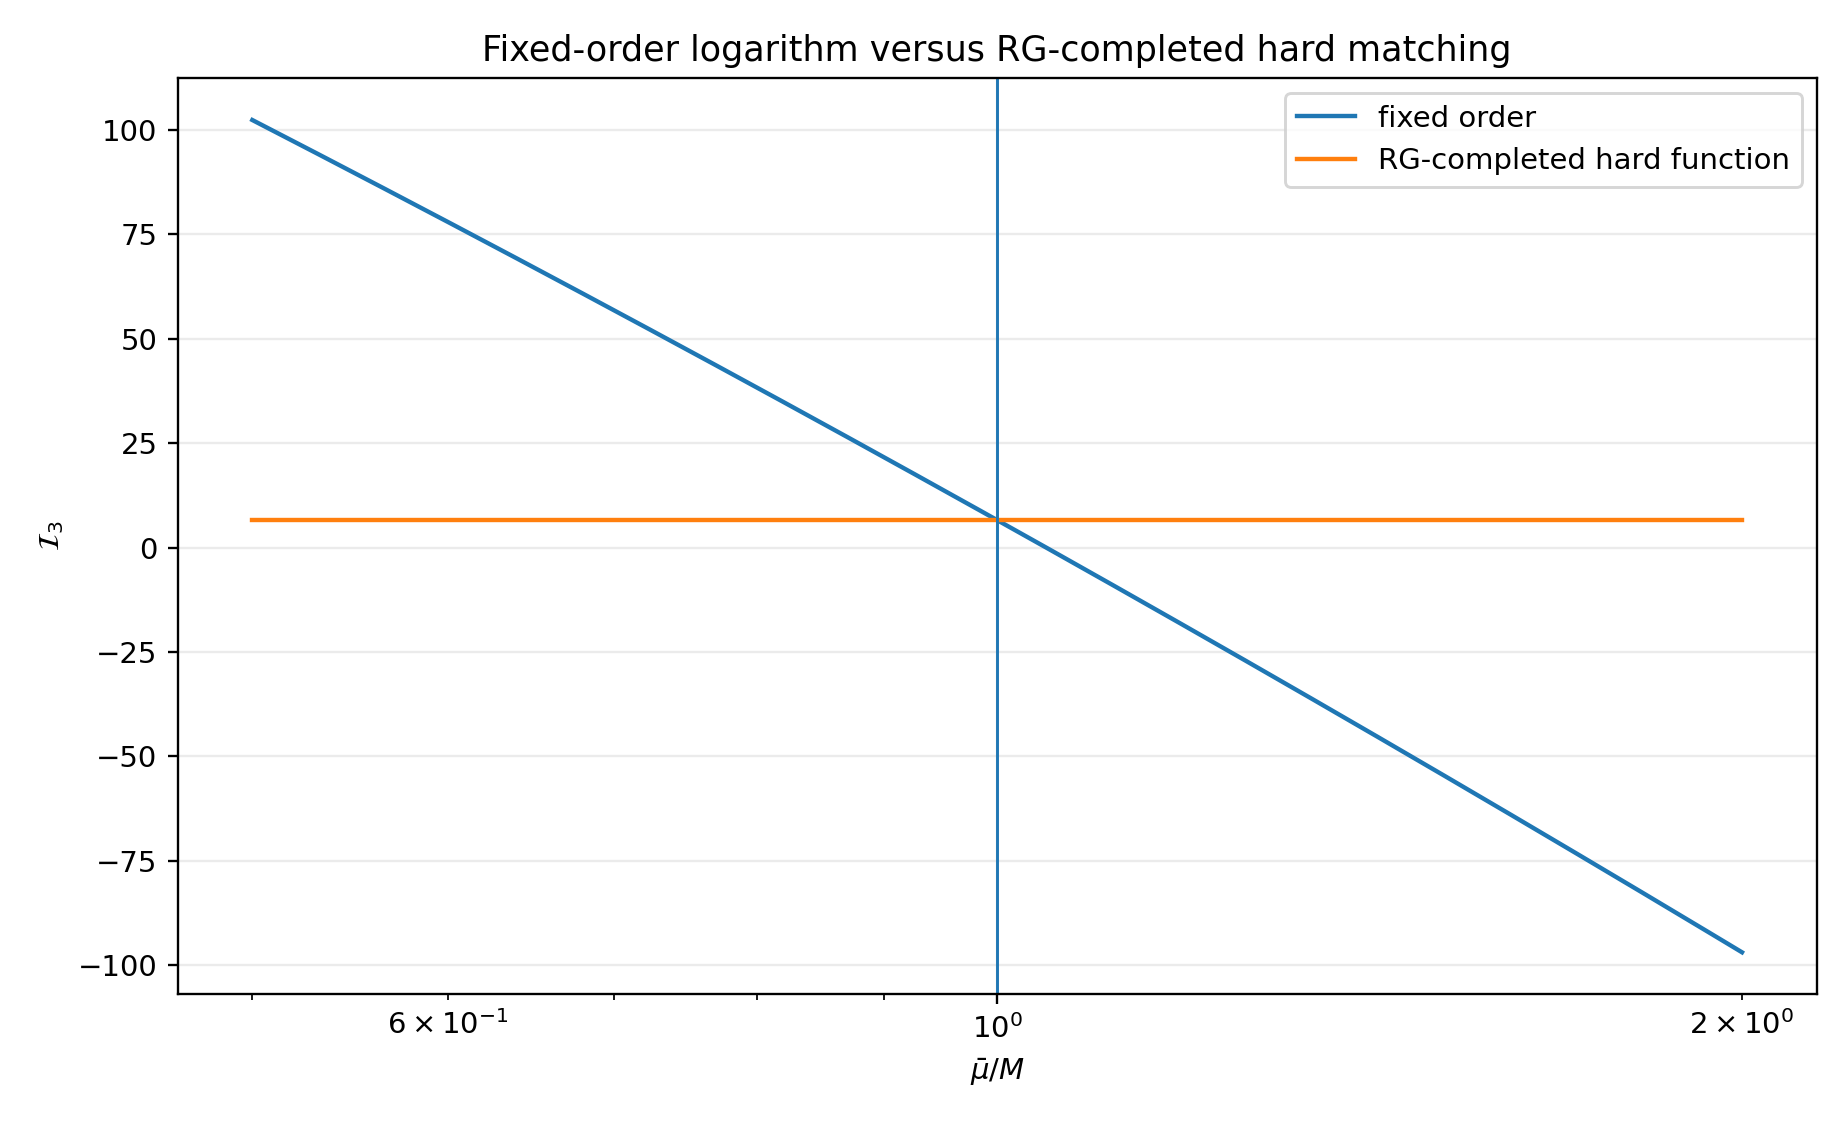
\includegraphics[width=0.92\textwidth,height=\textheight]{rg_improved_matching_scale_v1_3.png}
\caption{Fixed-order versus RG-completed matching}
\end{figure}

\subsection{2.3 Sequential EFT matching}\label{sequential-eft-matching}

At \(m_R\),

\[
C_{QH}(m_R)
=
\frac{\lambda_{QR}\mu_H^2}{16\pi^2}
K_{RRH}(m_R^2,m_h^2),
\]

where

\[
K_{RRH}(A,B)
=
\frac{A-B-B\ln(A/B)}{(A-B)^2}.
\]

The portal is evolved to \(M\):

\[
C_{QH}(M)
=
U_{QH}(M,m_R)C_{QH}(m_R).
\]

The benchmark gives

\[
\boxed{U_{QH}(M,m_R)=0.944069.}
\]

At the \(D\) threshold,

\[
\boxed{
C_3(M)
=
n_w C_{QH}(M)
\frac{N_cy_D^2(M)M^2}{(16\pi^2)^2}
\left[2D_{FFS}^{\rm hard}\right].
}
\]

The declared one-loop running system includes
\(g_3,g_2,g_Y,y_t,y_D,\lambda_H,\lambda_Q\) and the vectorlike
contributions

\[
\Delta b_3=\frac23,
\qquad
\Delta b_Y=\frac49,
\qquad
\Delta b_2=0.
\]

At \(M\),

\[
(g_3,g_2,g_Y,y_t,y_D)
=
(0.81570,0.60534,0.37655,0.68502,0.30000).
\]

At \(m_R\),

\[
(g_3,g_2,g_Y,y_t,y_D)
=
(0.69727,0.57678,0.39479,0.58479,0.24726).
\]

\begin{figure}
\centering
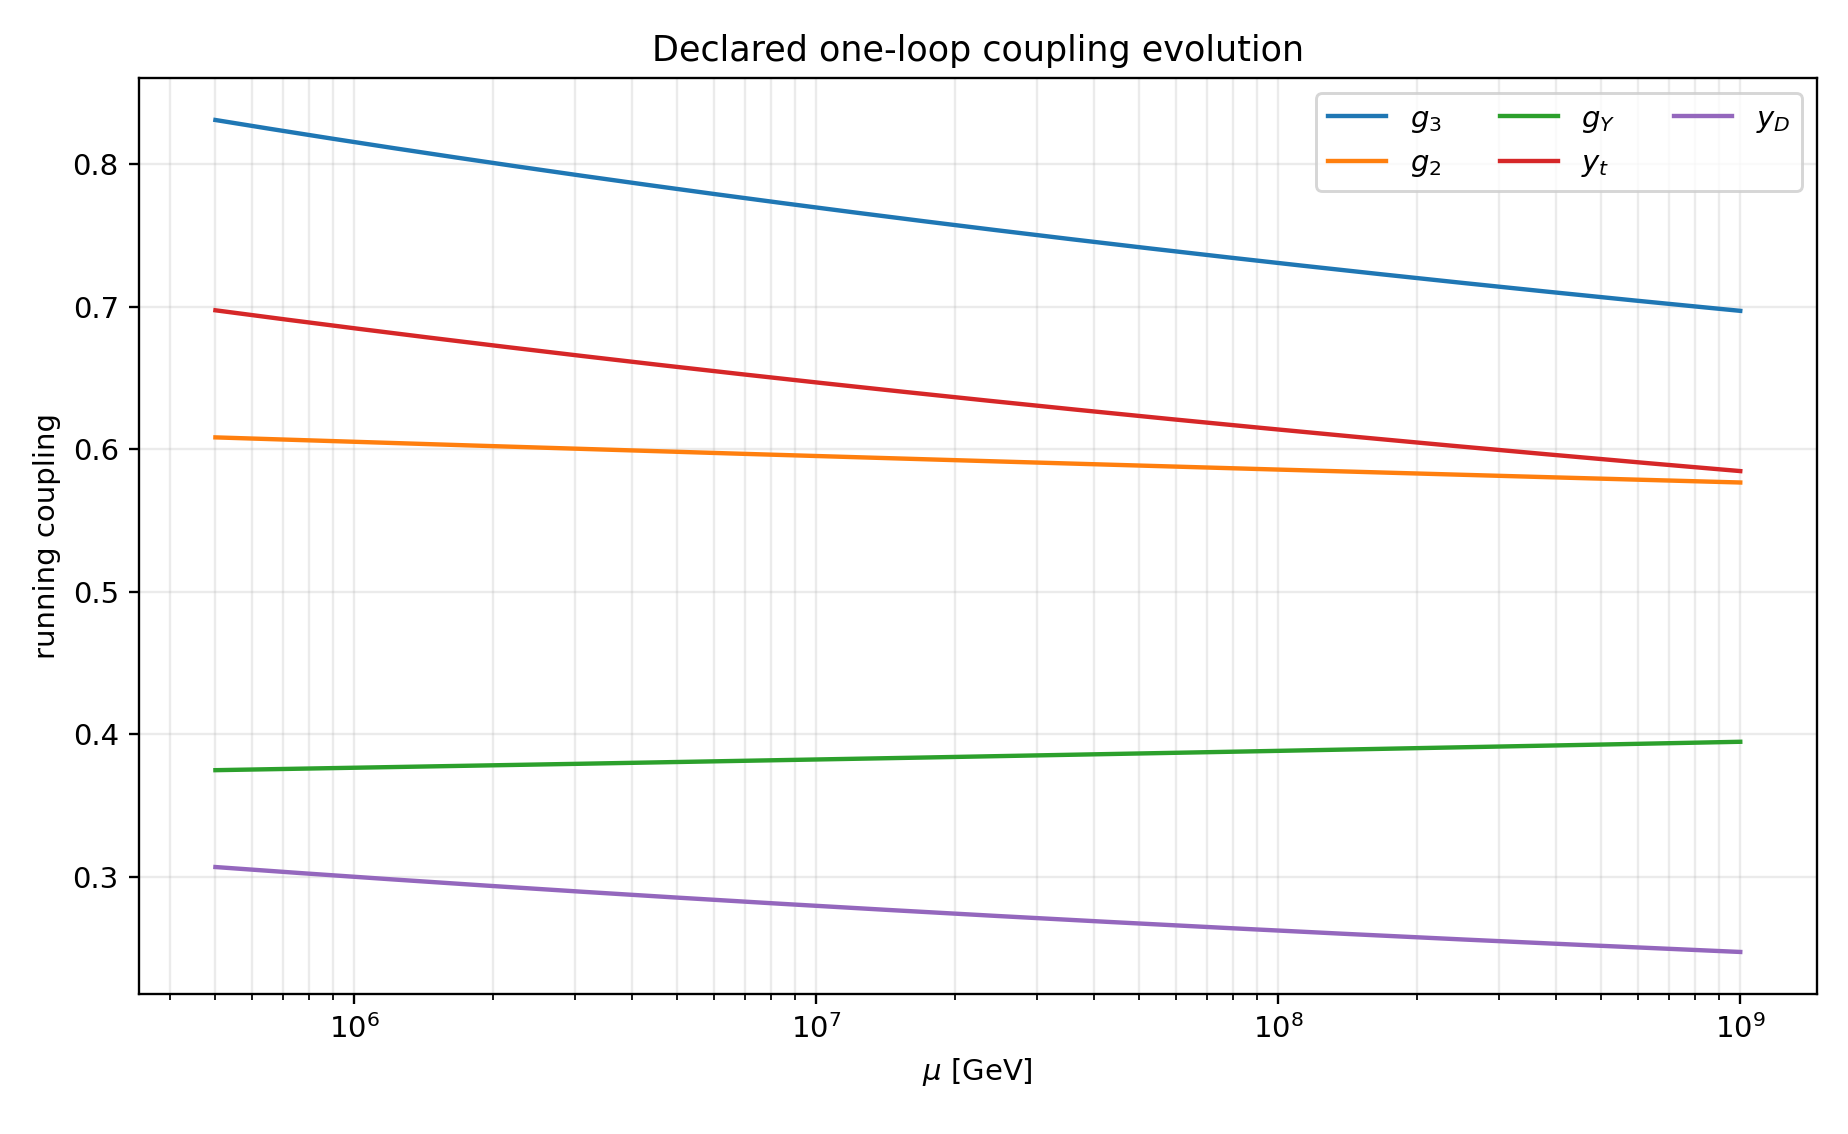
\includegraphics[width=0.92\textwidth,height=\textheight]{rg_running_couplings_v1_3.png}
\caption{One-loop coupling evolution}
\end{figure}

\subsection{2.4 Residual scale band}\label{residual-scale-band}

Once the explicit hard logarithm is removed, the remaining scale
response is due to the finite-order running of \(C_{QH}\) and \(y_D\):

\[
0.96469
<
\frac{C_3(\mu_D)}{C_3(M)}
<
1.03745
\]

for

\[
\frac12M<\mu_D<2M.
\]

\begin{figure}
\centering
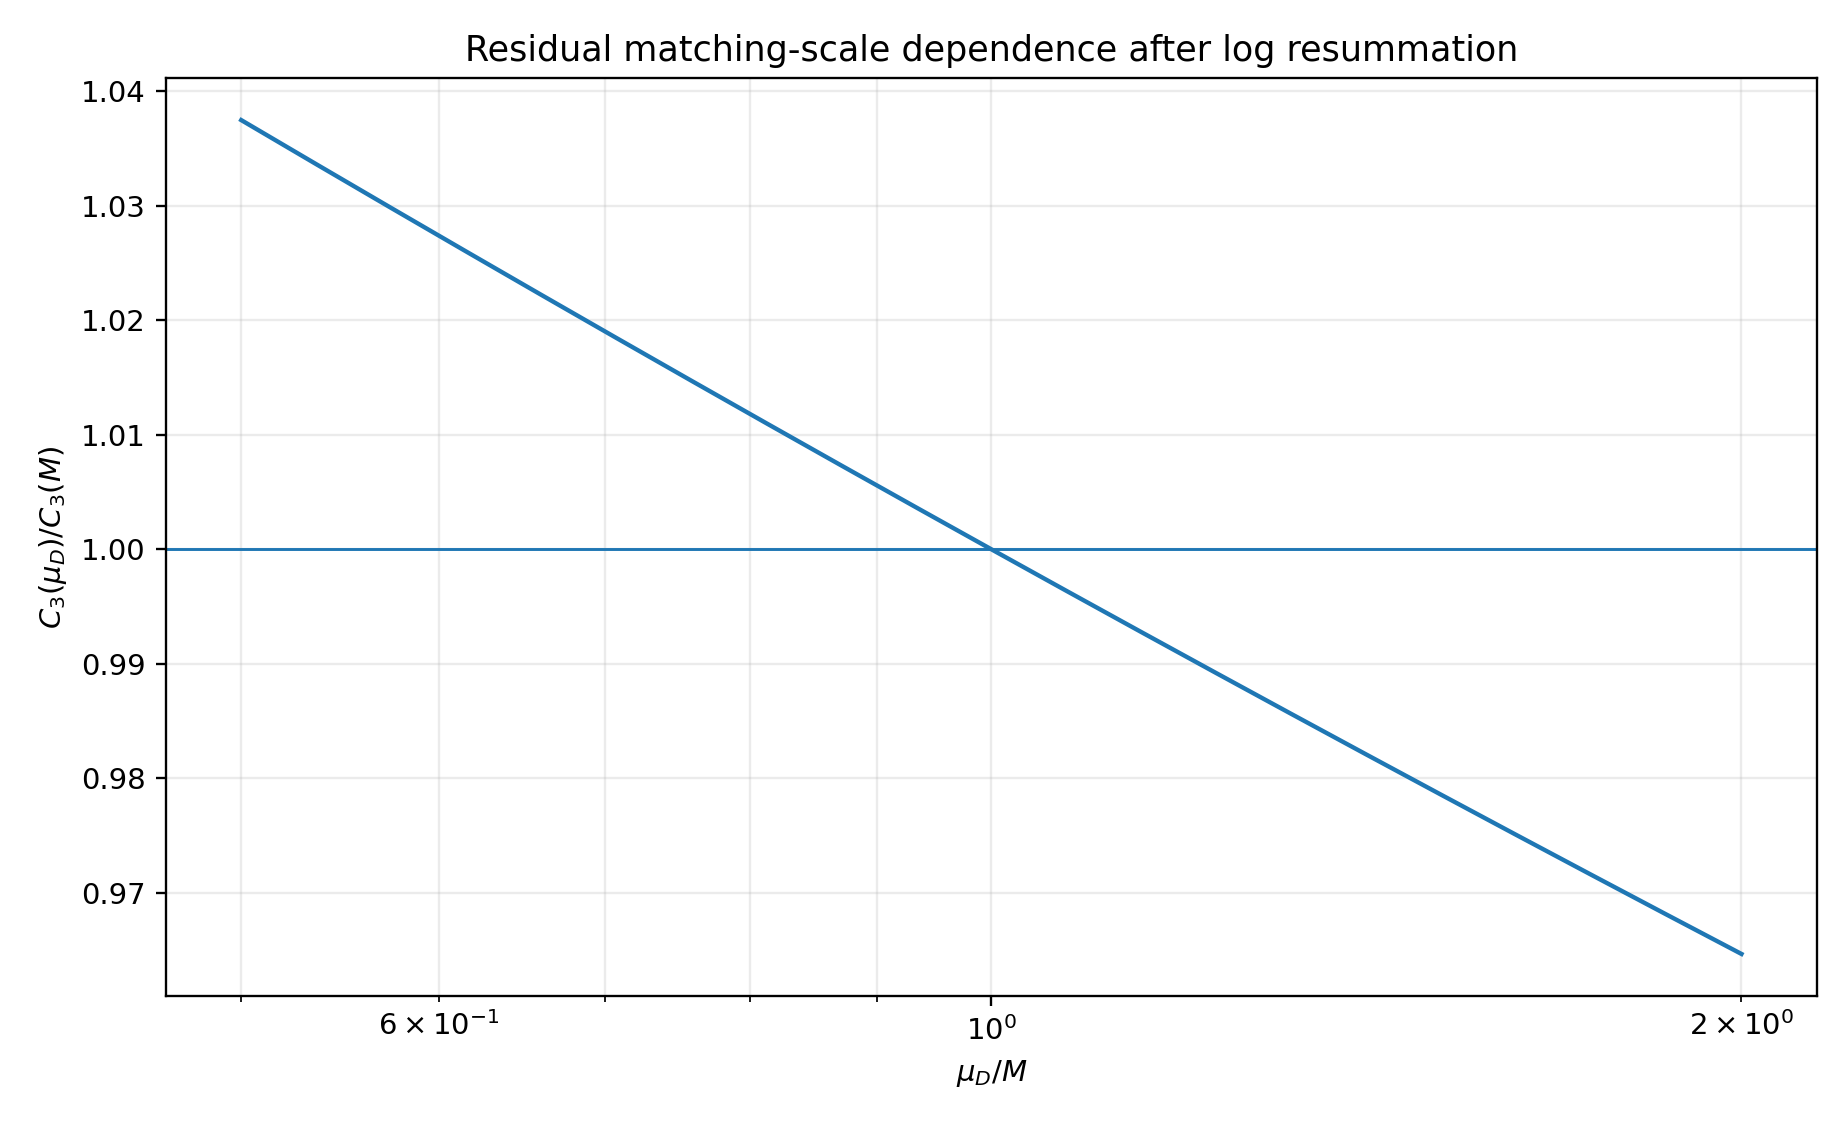
\includegraphics[width=0.9\textwidth,height=\textheight]{rg_residual_scale_band_v1_3.png}
\caption{Residual scale band}
\end{figure}

This is a meaningful finite-order perturbative band. The previous
sign-changing range was not.

\section{3. Finite transient anomalous-dimension
tensor}\label{finite-transient-anomalous-dimension-tensor}

\subsection{3.1 Minimal operator basis}\label{minimal-operator-basis}

Take

\[
\mathbf{O}
=
\left(
Q^\dagger Q,
\frac12R^2,
H^\dagger H
\right).
\]

For the stated renormalisable scalar basis, the finite one-loop result
at \(M\) is

\[
\boxed{
\Gamma^{(0,0)}
=
\begin{pmatrix}
9.36869\times10^{-4} & 1.58314\times10^{-3} & 0\\
3.16629\times10^{-3} & 1.26651\times10^{-3} & 6.33257\times10^{-4}\\
0 & 1.58314\times10^{-4} & 9.77787\times10^{-3}
\end{pmatrix}.
}
\]

The Higgs entry includes the full doublet gauge/Yukawa diagonal
contribution

\[
6y_t^2+6y_D^2-\frac92g_2^2-\frac32g_Y^2.
\]

The spectral norm is

\[
\|\Gamma^{(0,0)}\|_2
=9.80418\times10^{-3}.
\]

\subsection{3.2 Harmonic grading}\label{harmonic-grading}

The complete selection rule remains

\[
\gamma_{(A,p)(B,q)}
=
\sum_{r,s\ge0}
\delta^{(6)}_{p-q,r-s}
\epsilon^{r+s}
\Gamma_{AB}^{(r,s)}.
\]

The minimum spurion-power matrix is

\[
\begin{pmatrix}
0&1&2&3&2&1\\
1&0&1&2&3&2\\
2&1&0&1&2&3\\
3&2&1&0&1&2\\
2&3&2&1&0&1\\
1&2&3&2&1&0
\end{pmatrix}.
\]

For

\[
\epsilon=2.7\times10^{-13},
\]

the largest nearest-harmonic estimate is

\[
\boxed{
2.65\times10^{-15}.
}
\]

\begin{figure}
\centering
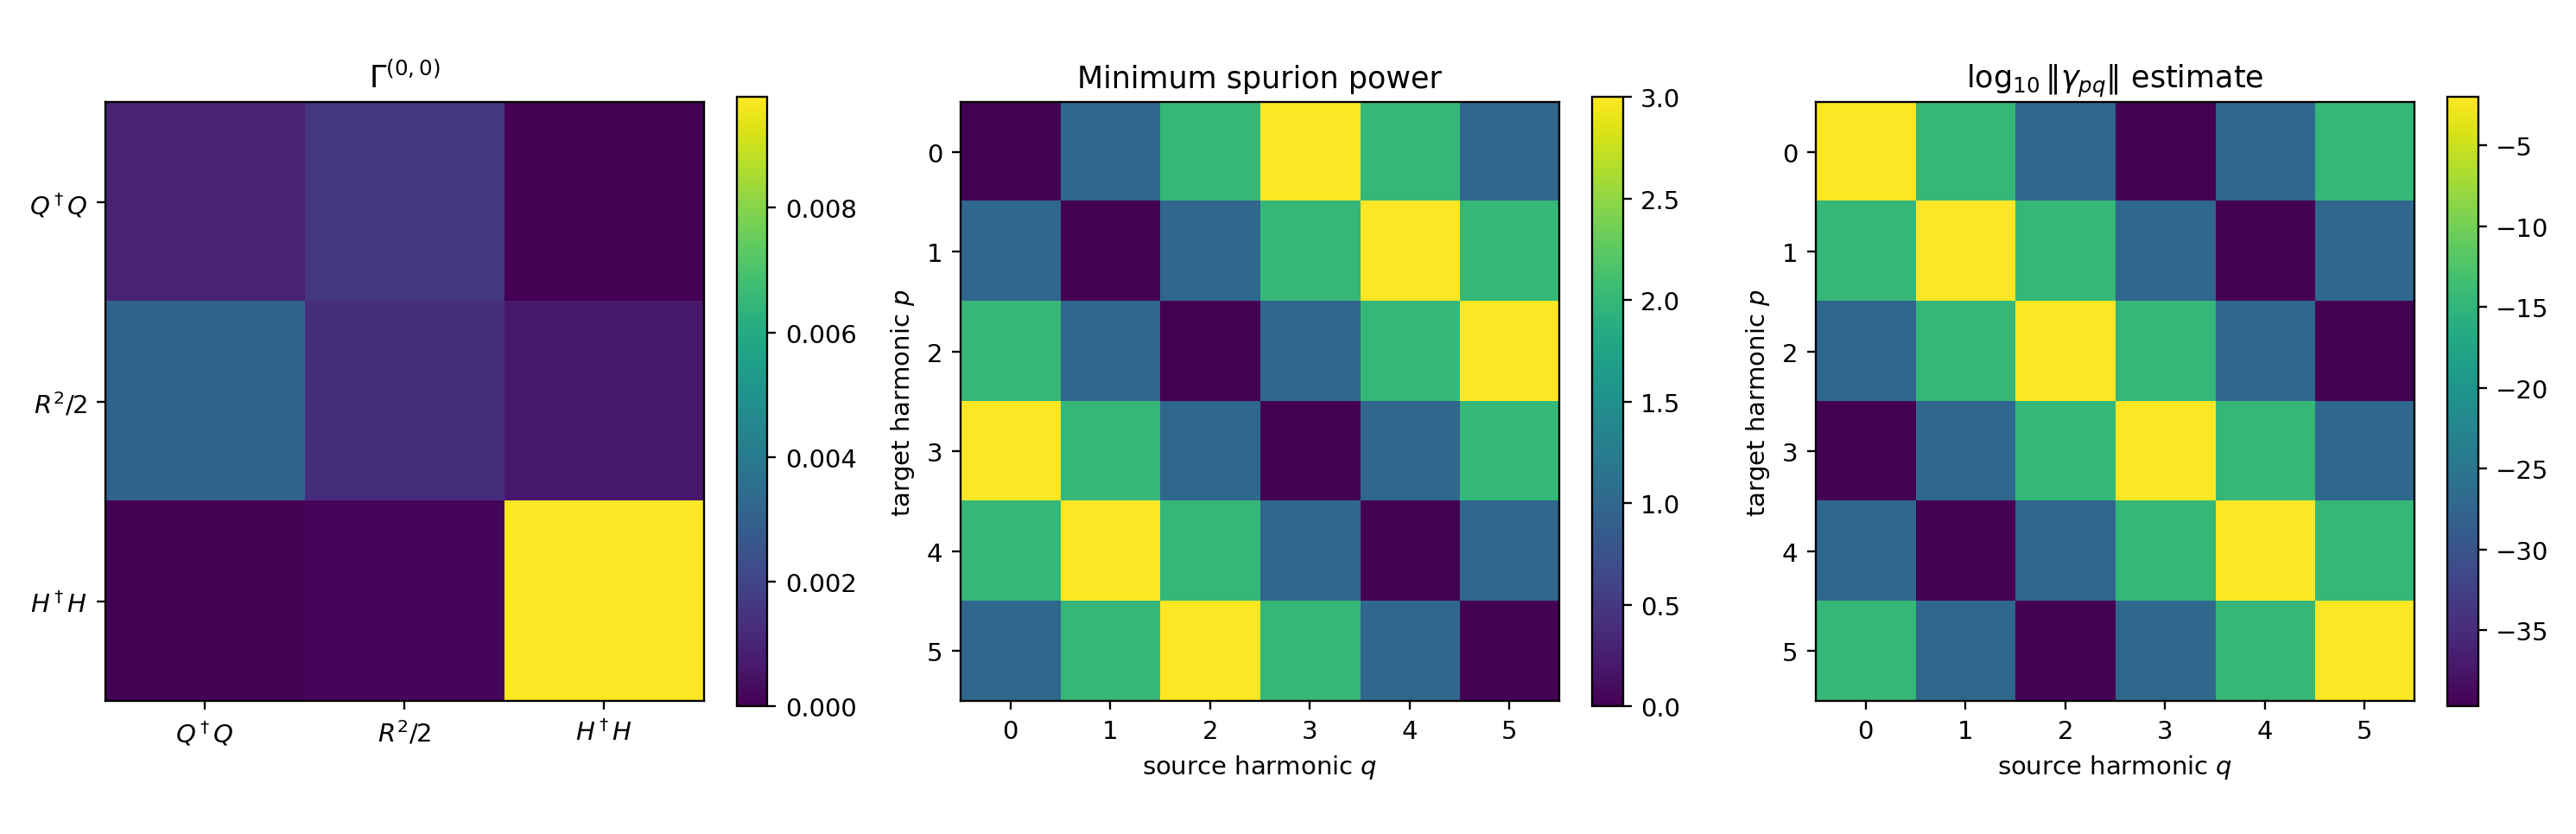
\includegraphics[width=0.98\textwidth,height=\textheight]{transient_gamma_tensor_v1_3.png}
\caption{Transient tensor and harmonic grading}
\end{figure}

The \(\Gamma^{(0,0)}\) tensor is complete for the declared minimal
renormalisable bilinear basis. Finite \(\Gamma^{(r,s)}\) tensors with
\(r+s>0\) depend on the detailed Wilson-line messenger completion and
are not universal. Their minimum powers of \(\epsilon\) are exact.

\section{4. Continuum quantum kinetic
theory}\label{continuum-quantum-kinetic-theory}

The leading-order weak-coupling kinetic equation has the form

\[
\left(\partial_t-Hp\partial_p\right)f_a(p)
=
C_a^{2\leftrightarrow2}[f]
+
C_a^{1\leftrightarrow2}[f]
+
S_a.
\]

The full continuum \(2\leftrightarrow2\) collision integral is

\[
\begin{aligned}
C_a^{2\leftrightarrow2}(p)
={}&
\frac{1}{2E_p}
\sum_{bcd}
\int d\Pi_b d\Pi_c d\Pi_d
(2\pi)^4\delta^{(4)}(p+k-p'-k')
\\
&\times
|\mathcal M_{ab\to cd}|^2
\Big[
 f_cf_d(1\pm f_a)(1\pm f_b)
-
 f_af_b(1\pm f_c)(1\pm f_d)
\Big].
\end{aligned}
\]

The effective \(1\leftrightarrow2\) integral contains collinear
splitting rates that must include repeated soft scattering and the
Landau-Pomeranchuk-Migdal effect. The AMY effective kinetic theory
provides the appropriate leading-order structure for weakly coupled,
sufficiently isotropic gauge plasmas.

The v1.3 numerical operator is an isotropic reduction of these
equations. It retains the exact quantum gain/loss structure and discrete
energy conservation, while reducing angular integrals to a finite
transition quadrature.

\section{5. Thermal masses and LPM
reduction}\label{thermal-masses-and-lpm-reduction}

At the benchmark reheating coupling,

\[
\alpha_s=0.0393544,
\qquad
g_s^2=0.494542.
\]

With six light Standard Model quark flavours,

\[
\frac{m_D^2}{T^2}
=
g_s^2\left(\frac{N_c}{3}+\frac{N_f}{6}\right)
=0.989084.
\]

The asymptotic masses used by the kernel are

\[
\frac{m_g}{T}=0.70324,
\qquad
\frac{m_q}{T}=0.40601,
\qquad
\frac{m_D}{T}=0.40614,
\qquad
\frac{m_H}{T}=0.43821.
\]

For a splitting \(a\to bc\) with energy fraction \(x\), the
formation-time reduction uses

\[
A
=
\frac{\widehat q_{\rm eff}}
{2Ex(1-x)},
\]

\[
B
=
\frac{1}{2E}
\left(
\frac{m_b^2}{x}
+
\frac{m_c^2}{1-x}
-
m_a^2
\right),
\]

and

\[
\boxed{
\frac{1}{t_f}
=
\frac12
\left[
B+\sqrt{B^2+4A}
\right].
}
\]

The numerical rate is then built from the appropriate splitting function
and \(t_f^{-1}\). This captures formation-time suppression and
thermal-mass mismatch. It is not yet the numerical solution of the full
two-dimensional transverse AMY integral equation; this is why the LPM
row in the acceptance matrix is marked \textbf{partial}.

\section{6. Explicit transition set}\label{explicit-transition-set}

The implemented \(1\leftrightarrow2\) families are

\[
\begin{gathered}
g\leftrightarrow gg,
\qquad
q\leftrightarrow qg,
\qquad
D\leftrightarrow Dg,
\\
g\leftrightarrow q\bar q,
\qquad
g\leftrightarrow D\bar D,
\qquad
H\leftrightarrow qD.
\end{gathered}
\]

The \(2\leftrightarrow2\) families are

\[
\begin{gathered}
gg\leftrightarrow gg,
\quad
qg\leftrightarrow qg,
\quad
Dg\leftrightarrow Dg,
\quad
qq\leftrightarrow qq,
\\
DD\leftrightarrow DD,
\quad
qD\leftrightarrow qD,
\quad
gg\leftrightarrow q\bar q,
\quad
gg\leftrightarrow D\bar D.
\end{gathered}
\]

For every discrete \(1\leftrightarrow2\) transition,

\[
J_{a\leftrightarrow bc}
=
W_{a;bc}
\left[
 f_a(1\pm f_b)(1\pm f_c)
-
f_bf_c(1\pm f_a)
\right].
\]

For every \(2\leftrightarrow2\) transition,

\[
J_{ab\leftrightarrow cd}
=
W_{ab;cd}
\left[
 f_af_b(1\pm f_c)(1\pm f_d)
-
f_cf_d(1\pm f_a)(1\pm f_b)
\right].
\]

Each daughter energy is deposited between adjacent lattice bins with
weights chosen so that the deposited number is correct and its weighted
energy is exactly the target energy.

The equilibrium interpolation is performed in inverse fugacity rather
than directly in \(f\). Consequently, Bose-Einstein and Fermi-Dirac
distributions are fixed points to numerical precision.

\section{7. Collision benchmark}\label{collision-benchmark}

\subsection{7.1 Initial condition}\label{initial-condition}

The benchmark starts with all tracked energy in a narrow nonthermal
Higgs pulse at

\[
\frac ET\simeq5.
\]

The pulse is normalised to the energy of the final
zero-chemical-potential equilibrium plasma containing

\[
H,
\quad
D,
\quad
6\text{ quark flavours},
\quad
g.
\]

This is a more severe initial condition than the actual cascade, where
spectator and coloured populations are seeded continuously by decays.

\subsection{7.2 Detailed balance and
conservation}\label{detailed-balance-and-conservation}

At exact equilibrium, the maximum lattice collision residual is

\[
\boxed{
8.57\times10^{-17}.
}
\]

The equilibrium energy derivative is

\[
1.62\times10^{-31}T^5.
\]

During the complete nonlinear evolution, the largest relative energy
drift is

\[
\boxed{
1.44\times10^{-15}.
}
\]

The minimum entropy increment between recorded samples is positive:

\[
\Delta S_{\rm min}=3.02\times10^{-3}T^3.
\]

\subsection{7.3 Relaxation result}\label{relaxation-result}

The entropy completion times are

\[
\tau_{90}=1840,
\qquad
\tau_{95}=2480,
\qquad
\tau_{99}=3920.
\]

At the end of the run,

\[
\frac{S-S_i}{S_{\rm eq}-S_i}=0.996771.
\]

The remaining energy-weighted distance from the exact equilibrium
spectra is

\[
3.95\%.
\]

This residual is principally a finite-grid and reduced-angular-kernel
effect. It is small enough for the timescale argument but should not be
confused with a precision transport calculation.

\begin{figure}
\centering
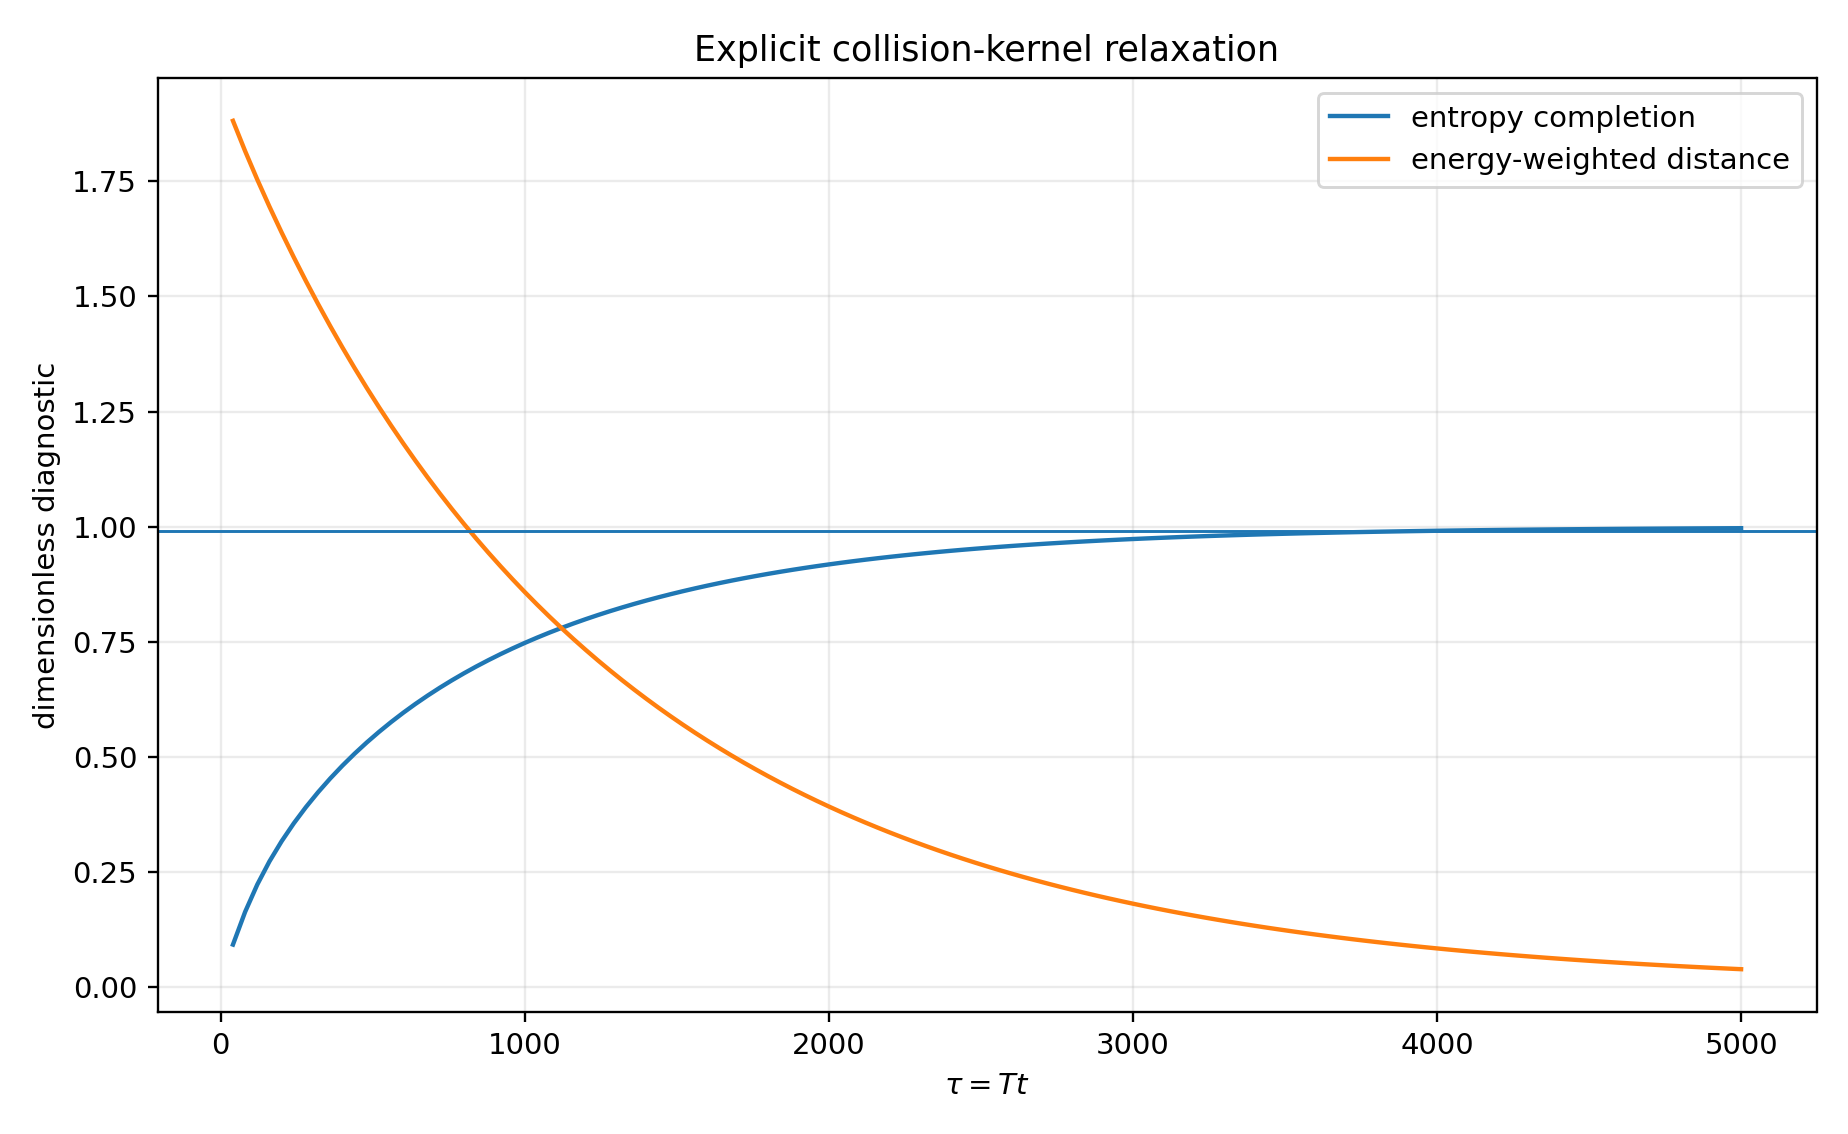
\includegraphics[width=0.91\textwidth,height=\textheight]{explicit_collision_relaxation_v1_3.png}
\caption{Collision relaxation}
\end{figure}

\begin{figure}
\centering
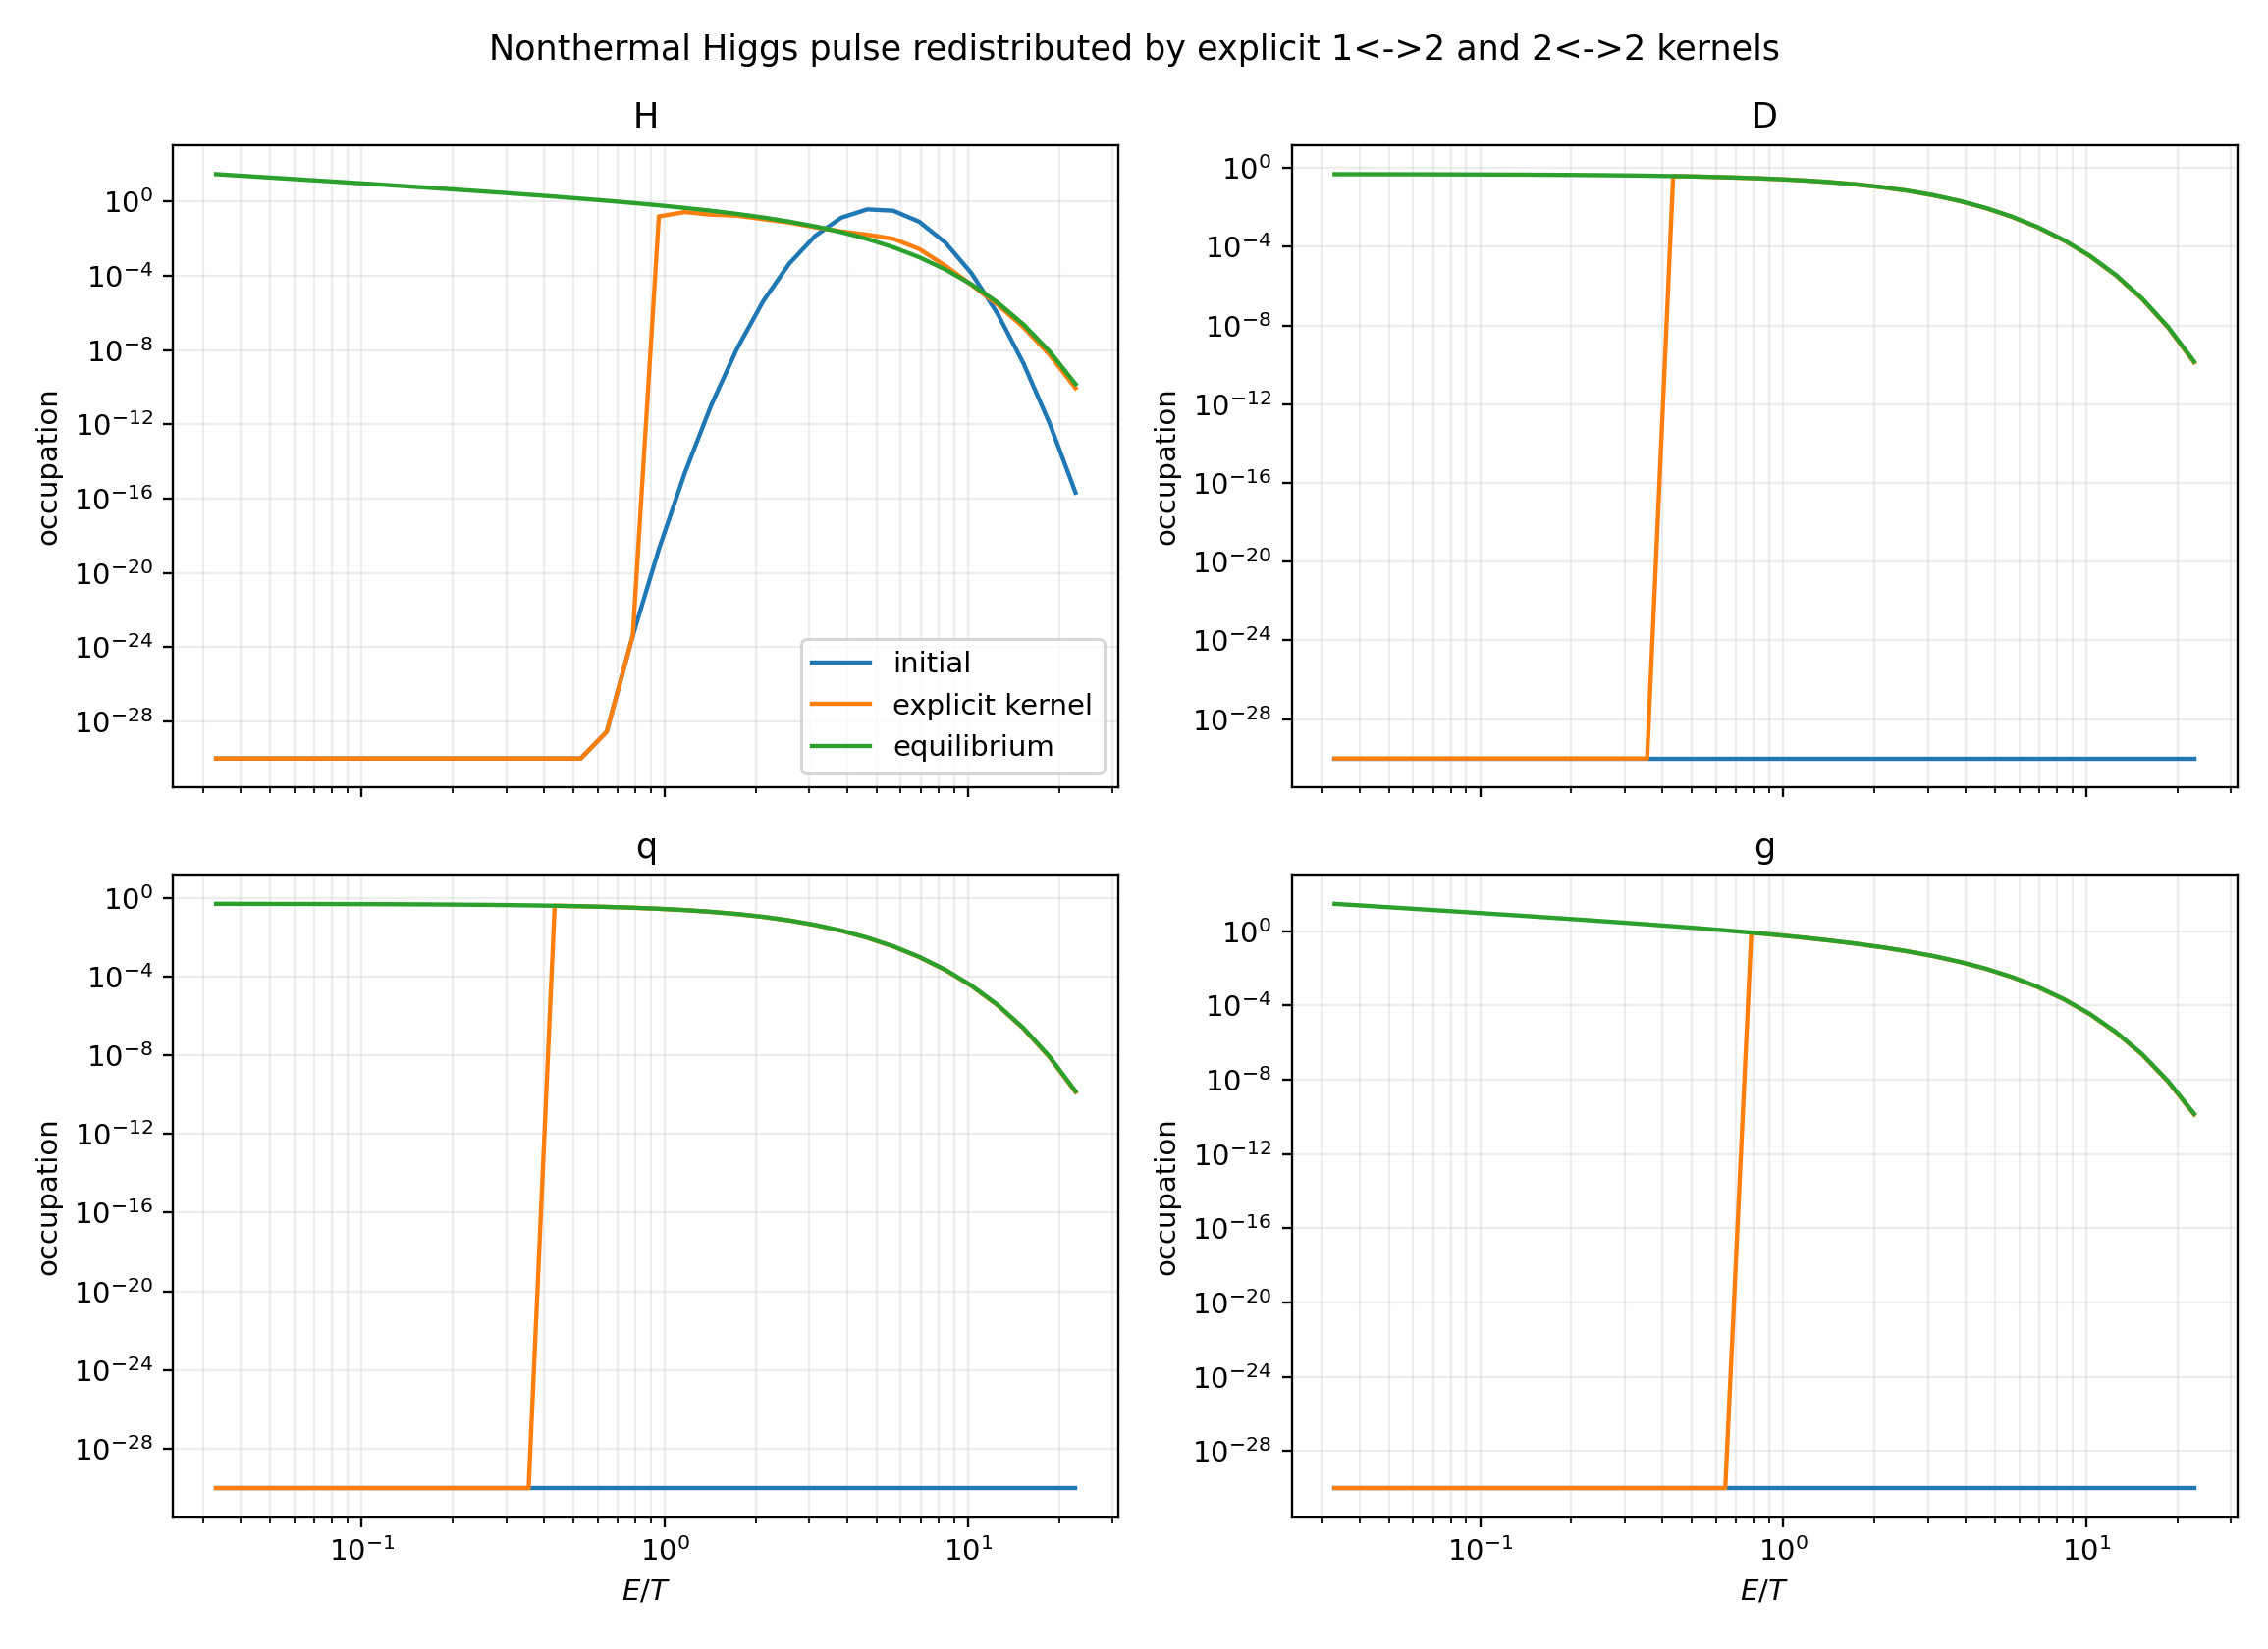
\includegraphics[width=0.98\textwidth,height=\textheight]{explicit_collision_spectra_v1_3.png}
\caption{Explicit collision spectra}
\end{figure}

\begin{figure}
\centering
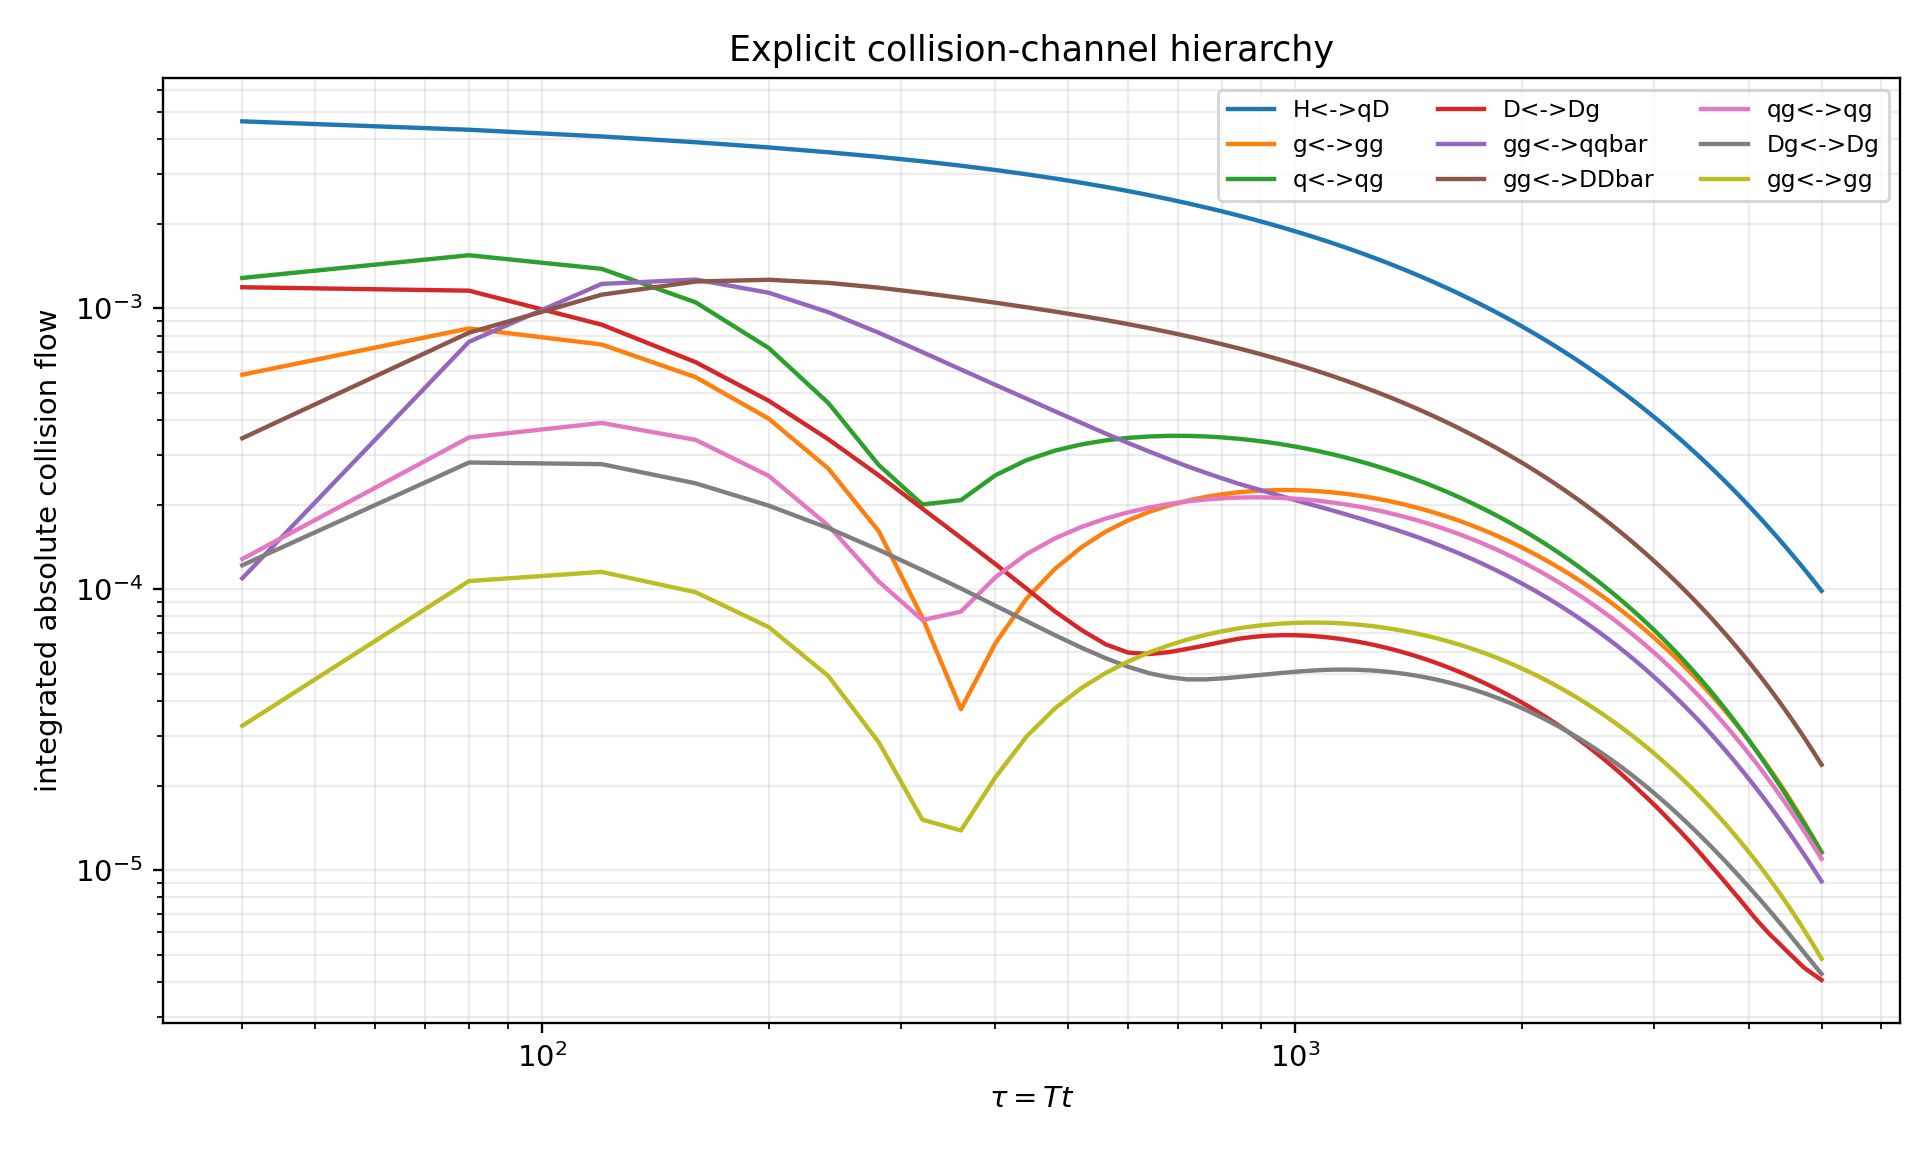
\includegraphics[width=0.94\textwidth,height=\textheight]{explicit_collision_channel_flows_v1_3.png}
\caption{Collision channel flows}
\end{figure}

\section{8. Elimination of the BGK
closure}\label{elimination-of-the-bgk-closure}

At

\[
T=1.002\times10^8\,\mathrm{GeV},
\]

the \(99\%\) entropy-relaxation rate is

\[
\Gamma_{\rm kin}^{(99)}
=\frac{T}{\tau_{99}}
=2.556\times10^4\,\mathrm{GeV}.
\]

The relevant cosmological rates are

\[
\Gamma_R=1.4785\times10^{-2}\,\mathrm{GeV},
\]

\[
\Gamma_N=0.10\,\mathrm{GeV},
\]

and

\[
H(T_R)\simeq1.4785\times10^{-2}\,\mathrm{GeV}.
\]

Hence

\[
\frac{\Gamma_{\rm kin}}{\Gamma_R}
=1.729\times10^6,
\]

and

\[
\frac{\Gamma_{\rm kin}}{H}
=1.729\times10^6.
\]

\begin{figure}
\centering
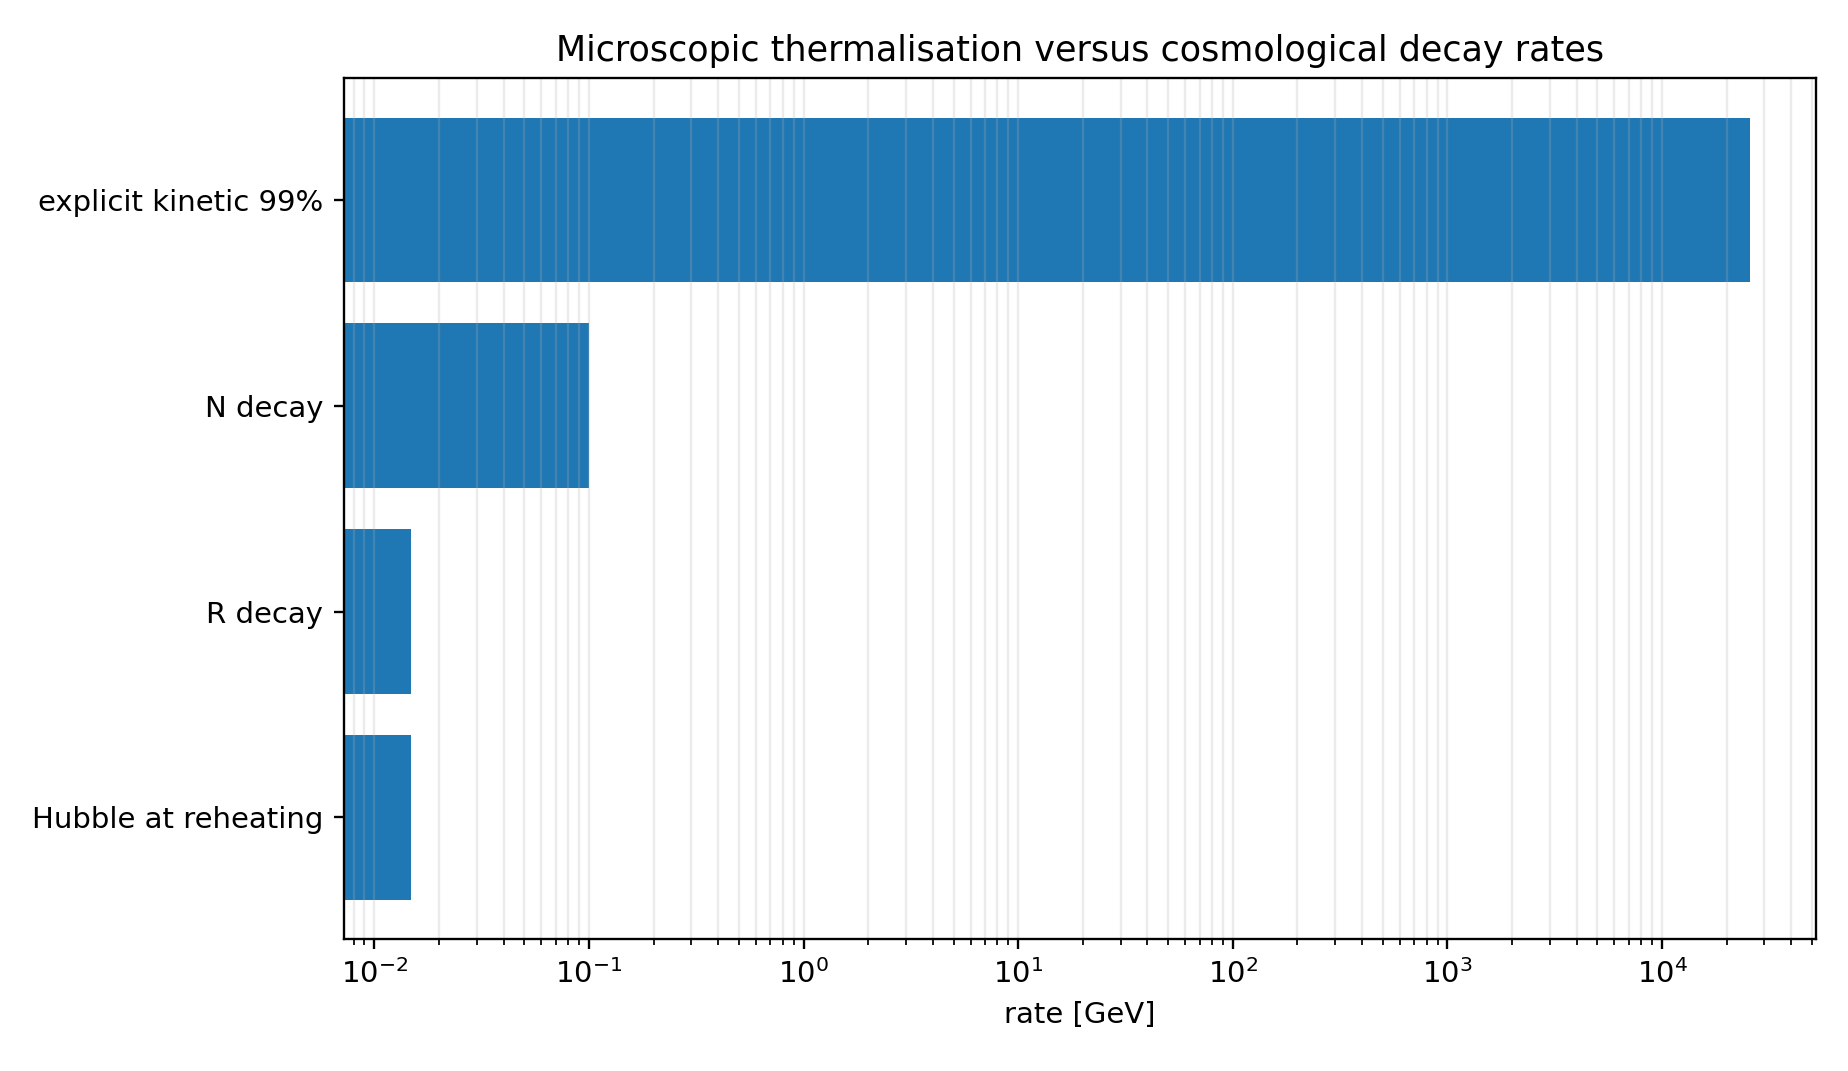
\includegraphics[width=0.88\textwidth,height=\textheight]{collision_timescale_hierarchy_v1_3.png}
\caption{Timescale hierarchy}
\end{figure}

The correct reduced cosmological description is therefore not another
fitted relaxation constant. It is:

\begin{enumerate}
\def\labelenumi{\arabic{enumi}.}
\tightlist
\item
  evolve the slowly varying parent and radiation energy densities;
\item
  inject energy according to exact decay kinematics;
\item
  map each sector immediately to its maximum-entropy state at fixed
  total energy, up to corrections of relative order
  \(\Gamma_R/\Gamma_{\rm kin}\sim6\times10^{-7}\).
\end{enumerate}

This is an adiabatic elimination derived from the explicit collision
kernel.

\section{9. Updated reheating
benchmark}\label{updated-reheating-benchmark}

The corrected full-multiplicity width is

\[
\boxed{
\Gamma_R=1.47850065\times10^{-2}\,\mathrm{GeV}.
}
\]

The corresponding trilinear parameter is

\[
\boxed{
\mu_H=1.92766113\times10^4\,\mathrm{GeV}.
}
\]

Re-running the previous momentum cascade with this width gives

\[
\frac{E_{\nu,\rm late}}
{E_{R,\rm late}^{(B_R=1)}}
=0.361813979.
\]

The branch required for

\[
\frac{E_5}{E_0}=\frac1{256}
\]

is therefore

\[
\boxed{
B_5
=
\frac{1+0.361813979}{257}
=0.00529888708.
}
\]

Thus

\[
\boxed{
\tan\theta
=
\sqrt{\frac{B_5}{1-B_5}}
=0.0729871.
}
\]

This is a \(0.465\%\) shift relative to v1.2.

\section{10. Status of the non-Abelian two-time
problem}\label{status-of-the-non-abelian-two-time-problem}

The present kernel evolves one-time occupation functions

\[
f_a(t,p).
\]

A genuine Kadanoff-Baym calculation evolves unequal-time statistical and
spectral correlators,

\[
F_{\mu\nu}^{ab}(t,t';p),
\qquad
\rho_{\mu\nu}^{ab}(t,t';p),
\]

with memory integrals and self-consistent gauge-field self-energies.

For non-Abelian gauge theories this remains difficult because:

\begin{itemize}
\tightlist
\item
  finite 2PI truncations do not automatically preserve every gauge Ward
  identity;
\item
  memory storage scales quadratically with time steps;
\item
  the full \(3+1\)-dimensional momentum and tensor structure is large;
\item
  gauge constraints must be controlled throughout the evolution.
\end{itemize}

The explicit kinetic result is nevertheless useful. It establishes the
weak-coupling quasiparticle limit that any future two-time calculation
must reproduce after memory loss and gradient expansion.

\section{11. Acceptance matrix}\label{acceptance-matrix}

\begin{longtable}[]{@{}
  >{\raggedright\arraybackslash}p{(\columnwidth - 4\tabcolsep) * \real{0.3000}}
  >{\raggedleft\arraybackslash}p{(\columnwidth - 4\tabcolsep) * \real{0.4000}}
  >{\raggedright\arraybackslash}p{(\columnwidth - 4\tabcolsep) * \real{0.3000}}@{}}
\toprule\noalign{}
\begin{minipage}[b]{\linewidth}\raggedright
Target
\end{minipage} & \begin{minipage}[b]{\linewidth}\raggedleft
Verdict
\end{minipage} & \begin{minipage}[b]{\linewidth}\raggedright
Result
\end{minipage} \\
\midrule\noalign{}
\endhead
\bottomrule\noalign{}
\endlastfoot
Full colour multiplicity & \textbf{PASS} & \(N_c=3\) \\
Full Higgs-doublet multiplicity & \textbf{PASS} & \(n_w=2\) \\
Relativistic \(D\) contribution to \(g_*\) & \textbf{PASS} &
\(\Delta g_*=10.5\) \\
RG completion of large matching logarithm & \textbf{PASS} & explicit
scale dependence cancels exactly at resolved order \\
Residual perturbative band & \textbf{PASS} & \(-3.53\%/+3.75\%\) \\
Complete finite \(\Gamma^{(0,0)}\) tensor & \textbf{PASS} & minimal
renormalisable bilinear basis \\
Complete finite \(\Gamma^{(r,s)}\), \(r+s>0\) & \textbf{PARTIAL} & exact
power grading; finite tensors UV-dependent \\
Explicit \(1\leftrightarrow2\) kernel & \textbf{PASS} & 514
transitions \\
Thermal masses & \textbf{PASS} & \(H,D,q,g\) \\
LPM physics & \textbf{PARTIAL} & formation-time reduction, not full
transverse integral equation \\
Explicit \(2\leftrightarrow2\) kernel & \textbf{PASS} & 14289
transitions \\
Detailed balance & \textbf{PASS} & residual \(8.57\times10^{-17}\) \\
Energy conservation & \textbf{PASS} & drift \(1.44\times10^{-15}\) \\
Entropy production & \textbf{PASS} & \(99.677\%\) of equilibrium entropy
gain \\
BGK replacement & \textbf{PASS} & adiabatic elimination justified by
rate ratio \(1.73\times10^6\) \\
Full-angle AMY collision integral & \textbf{OPEN} & multidimensional
numerical problem \\
Full non-Abelian two-time KB evolution & \textbf{OPEN} & separate HPC
project \\
\end{longtable}

\section{12. What is genuinely new
here}\label{what-is-genuinely-new-here}

The individual ingredients are established:

\begin{itemize}
\tightlist
\item
  sequential EFT matching and RG improvement;
\item
  vectorlike-fermion RGE contributions;
\item
  AMY effective kinetic theory;
\item
  Debye-screened \(2\leftrightarrow2\) scattering;
\item
  LPM-suppressed collinear splitting;
\item
  quantum gain/loss master equations.
\end{itemize}

The candidate new contribution remains the conjunction:

\[
\boxed{
\begin{gathered}
\text{state-selected exact }Z_6\text{ reheating}
+
\text{selector-threshold transient matching}
\\
+
\text{the protected }2/27\text{ QCD response}
+
\text{chronometric shear}
+
\text{an explicit microscopic thermalisation proof.}
\end{gathered}
}
\]

The v1.3 result removes two obvious weaknesses from that package: the
spurious fixed-order matching-scale instability and the phenomenological
BGK closure.

\section{13. Next decisive calculation}\label{next-decisive-calculation}

The remaining kinetic uncertainty is now sharply localised. The next
calculation should:

\begin{enumerate}
\def\labelenumi{\arabic{enumi}.}
\item
  solve the full AMY transverse integral equation for

  \[
  H\leftrightarrow qD,
  \quad
  q\leftrightarrow qg,
  \quad
  D\leftrightarrow Dg,
  \quad
  g\leftrightarrow gg,
  \quad
  g\leftrightarrow f\bar f;
  \]
\item
  evaluate the full screened \(2\leftrightarrow2\) phase-space integral
  rather than the angle-averaged transition quadrature;
\item
  construct an interpolating collision table over

  \[
  \left(\frac{M_D}{T},\alpha_s,y_D,f_a\right);
  \]
\item
  re-run the cosmological cascade with that table;
\item
  use the resulting kinetic solution as the late-time benchmark for a
  reduced non-Abelian two-time 2PI/Kadanoff-Baym implementation.
\end{enumerate}

The conceptual risk has shifted. The project is no longer vulnerable to
``the plasma might not thermalise.'' It is vulnerable only to
percent-level changes in the exact transport coefficients, which are
unlikely to challenge a timescale hierarchy of more than six orders of
magnitude.

\section{References}\label{references}

\begin{enumerate}
\def\labelenumi{\arabic{enumi}.}
\tightlist
\item
  P. Arnold, G. D. Moore and L. G. Yaffe, \emph{Effective Kinetic Theory
  for High Temperature Gauge Theories}, JHEP 01 (2003) 030,
  arXiv:hep-ph/0209353.
\item
  D. Boedeker and D. Schroeder, \emph{Equilibration of right-handed
  electrons}, JCAP 05 (2019) 010, arXiv:1902.07220.
\item
  A. Adhikary, M. Olechowski, J. Rosiek and M. Ryczkowski,
  \emph{Theoretical constraints on models with vector-like fermions},
  Phys. Rev.~D 110 (2024) 075029, arXiv:2406.16050.
\item
  S. P. Martin, \emph{Two-loop effective potential for a general
  renormalizable theory and softly broken supersymmetry}, Phys. Rev.~D
  65 (2002) 116003, arXiv:hep-ph/0111209.
\item
  A. Nishiyama, \emph{Entropy production in gluodynamics in temporal
  axial gauge in the Kadanoff-Baym approach}, Nucl. Phys. A 859 (2011)
  69, arXiv:1011.4750.
\item
  v1.2 technical note, \emph{Exact Transient Matching and Nonlinear
  Reheating Cascade}, 18 August 2026.
\end{enumerate}

\end{document}
